%notar que ocupamos xcolor and dvipnames como variables globales, 
%pues al trabajar con svg tenemos que el paquete ya añade a xcolor y esto nos genera un cierto conflicto en el documento

%pdflatex --jobname=picture/t3/g_tam1.pdf

\documentclass[letterpaper,10pt,table, dvipsnames]{article}
\usepackage[vmargin=1.5cm,hmargin=2cm,head=30pt,includeheadfoot]{geometry}
\usepackage[spanish,es-tabla]{babel}
\usepackage[utf8]{inputenc}
\usepackage{graphicx}
\DeclareGraphicsExtensions{.jpg,.pdf,.mps,.png}
%Paquetes adicionales, ayudan para portada (algunos)
\usepackage{amssymb}
\usepackage{amsfonts}
\usepackage{amsmath}
\usepackage{fancyhdr}
\usepackage{wrapfig}
\usepackage{xcolor}
\colorlet{LightRubineRed}{RubineRed!70!}%https://www.overleaf.com/learn/latex/Using_colours_in_LaTeX
\usepackage{multicol}
\usepackage{changepage}
\usepackage{float}
\usepackage{array, makecell} %
\usepackage{tcolorbox}
\usepackage{enumitem}
\usepackage{tikz}
\usetikzlibrary{shapes.geometric}
\usetikzlibrary{babel,quotes,positioning,arrows,snakes,backgrounds,fit,trees,matrix}
\usepackage{tkz-graph}
\usepackage{rotating}
\usetikzlibrary{arrows.meta}

%https://tex.stackexchange.com/questions/455341/how-to-represent-the-shift-key
%https://tex.stackexchange.com/questions/176398/carriage-return-symbol-new-command
\usepackage{keystroke}
\usepackage{menukeys}
\usepackage{tabularx,ragged2e,booktabs,caption}
\captionsetup{%
  labelfont={bf,sf},      % label in bold, sans-serif
  singlelinecheck=true, % centered single-lined captions
  format=plain,             % indention=1cm,
  labelsep={colon},         % default separator: none, colon, period, space, quad, newline, endash
} 
\definecolor{gray51}{rgb}{0.51,0.51,0.51}
\definecolor{antiquewhite}{rgb}{0.98, 0.92, 0.84}
\definecolor{gainsboro}{rgb}{0.86, 0.86, 0.86}
\definecolor{isabelline}{rgb}{0.96, 0.94, 0.93}
\definecolor{bg}{HTML}{282828} % from https://github.com/kevinsawicki/monokai
%\definecolor{isabelline}{rgb}{1.0, 1.0, 1.0}

\usepackage{svg}

%https://tex.stackexchange.com/questions/55210/not-element-of-in-latin-modern


\usepackage{bigstrut}%paquete para tablas latex en excel

%%%%%%%%%%%%%%%%%%%%%%%%%%%%%%%%%%%%%%%%%%%%%%%%%%%%%%%
% Default fixed font does not support bold face
%\DeclareFixedFont{\ttb}{T1}{txtt}{bx}{n}{9.5} % for bold
%\DeclareFixedFont{\ttm}{T1}{txtt}{m}{n}{9.5}  % for normal
%
%%COLORS for listings
%\definecolor{deepblue}{rgb}{0,0,0.5}
%\definecolor{deepred}{rgb}{0.6,0,0}
%\definecolor{deepgreen}{rgb}{0,0.5,0}
%\definecolor{deeppurple}{rgb}{0.6, 0.2, 0.7}
%
%\usepackage{listings}
%\lstset{
%  backgroundcolor=\color{isabelline}, %color de fondo
%  %backgroundcolor=\color{gainsboro},
%  %breaklines=true,
%  captionpos=b,     % Establece la posición de la leyenda del cuadro de código
%  %basicstyle=\footnotesize,
%  commentstyle=\color{red},
%}

%%%%%%%%%%%%%%%%%%%% CONFIGURACION CON LISTING

%\newcommand\pythonstyle{\lstset{
%language=Python,
%numbers=left,
%numberstyle=\tiny,
%xleftmargin=2em,
%numberstyle=\footnotesize,
%basicstyle=\ttm,
%tabsize=4,
%otherkeywords={self},             % Add keywords here
%keywordstyle=\ttb\color{deepblue},
%emph={MyClass,__init__},          % Custom highlighting
%emphstyle=\ttb\color{deepred},    % Custom highlighting style
%stringstyle=\color{deepgreen},
%frame=tb,                         % Any extra options here
%showstringspaces=false            % 
%}}
%\renewcommand*{\lstlistingname}{\textbf{Código}}  %CAMBIA EL TITULO DE LISTING EN EL CODIGO

%%%%%%%%%%%%%%%%%

% Interlineado
\linespread{1.5}
\usepackage{hyperref}
\usepackage{natbib}
\setcitestyle{super}
\usepackage{blindtext}
\linespread{1.0}\selectfont

\usepackage{dsfont}
\fancypagestyle{style2}{
\fancyhf{}
\lhead{
\begin{wrapfigure}{l}{0.2\textwidth}
\vspace{-2.4cm}

\includegraphics[scale=0.2]{dcc_2019}
\end{wrapfigure}
  %\hspace*{0.3cm}
  %\textcolor{RubineRed}{\textsf{Liceo 1 Javiera Carrera}} \\
  %\hspace*{0.3cm}
  %\textcolor{gray51}{\textsc{Resumen Probabilidad N$^{o}$1}} % Licencia en la izquierda del encabezado
  %\vspace{0.6cm}
} % TITULO DEL ENSAYO
\rhead{\textsf{Universidad de Chile\\ Departamento de Ciencia de la Computación}\\
\textbf{\textsf{CC3102 Teoría de la Computación}}
\vspace{0.1cm}}
\renewcommand{\headrulewidth}{0.4pt}
}

\newcommand{\EXP}{\mathcal{EXP}}
%%%%%%%%%%%%%%%PARA LISTING
% Python environment
%\lstnewenvironment{python}[1][]
%{
%\pythonstyle
%\lstset{#1}
%}
%{}

%% Python for external files
%\newcommand\pythonexternal[2][]{{
%\pythonstyle
%%\lstinputlisting[#1]{#2}}}
%%
%% Python for inline
%\newcommand\pythoninline[1]{{\pythonstyle\lstinline!#1!}}
%%%%%%%%%%%%%%%%%%%%%%%%%%

\newcommand{\figref}[1]{\figurename~\ref{#1}}
\newcommand{\codref}[1]{\lstlistingname~\ref{#1}}

%suprime indentacion
\setlength\parindent{0pt}


\begin{document}

\pagestyle{style2}
\begin{figure}
\centering
\begin{minipage}[c]{0.8\textwidth}
\centering
\vspace{0.3cm}
{\Large Tarea 3}
\vspace{0.3cm}\\
\textbf{Profesor:} Alejandro Hevia \\ \textbf{Auxiliares:} Ivanna Bachmann, Rodrigo Fuentes, Vicente Rojas\\
\textbf{Alumno:} Sebastián Sepúlveda A.
\end{minipage}
\end{figure}

\textbf{{\Large Soluciones}}
\\

\begin{tcolorbox}
\boxed{\textbf{Problema 1.1}} Los strings sobre el alfabeto $\{0,1,2\}$ que representan, en base 3, a un número n, tal que n no es divisible por 9
\end{tcolorbox}

\begin{center}
\begin{tikzpicture}[scale=0.2]
\tikzstyle{every node}+=[inner sep=0pt]
\draw [black] (12.4,-31.6) circle (3);
\draw (12.4,-31.6) node {$q_0$};
\draw [black] (23.6,-19.1) circle (3);
\draw (23.6,-19.1) node {$q_1$};
\draw [black] (36.1,-13.9) circle (3);
\draw (36.1,-13.9) node {$q_f$};
\draw [black] (36.1,-13.9) circle (2.4);
\draw [black] (36.1,-23.5) circle (3);
\draw (36.1,-23.5) node {$q_f$};
\draw [black] (36.1,-23.5) circle (2.4);
\draw [black] (23.6,-43.3) circle (3);
\draw (23.6,-43.3) node {$q_2$};
\draw [black] (35,-34.4) circle (3);
\draw (35,-34.4) node {$q_f$};
\draw [black] (35,-34.4) circle (2.4);
\draw [black] (35,-43.3) circle (3);
\draw (35,-43.3) node {$q_f$};
\draw [black] (35,-43.3) circle (2.4);
\draw [black] (35,-51.8) circle (3);
\draw (35,-51.8) node {$q_f$};
\draw [black] (35,-51.8) circle (2.4);
\draw [black] (6.4,-31.6) -- (9.4,-31.6);
\fill [black] (9.4,-31.6) -- (8.6,-31.1) -- (8.6,-32.1);
\draw [black] (11.077,-28.92) arc (234:-54:2.25);
\draw (12.4,-24.35) node [above] {$0$};
\fill [black] (13.72,-28.92) -- (14.6,-28.57) -- (13.79,-27.98);
\draw [black] (14.4,-29.37) -- (21.6,-21.33);
\fill [black] (21.6,-21.33) -- (20.69,-21.6) -- (21.44,-22.26);
\draw (18.54,-26.81) node [right] {$0$};
\draw [black] (26.37,-17.95) -- (33.33,-15.05);
\fill [black] (33.33,-15.05) -- (32.4,-14.9) -- (32.78,-15.82);
\draw (28.88,-15.99) node [above] {$1$};
\draw [black] (26.43,-20.1) -- (33.27,-22.5);
\fill [black] (33.27,-22.5) -- (32.68,-21.77) -- (32.35,-22.71);
\draw (28.94,-21.83) node [below] {$2$};
\draw [black] (21.667,-16.821) arc (248.03624:-39.96376:2.25);
\draw (21.24,-11.98) node [above] {$0$};
\fill [black] (24.23,-16.18) -- (25,-15.62) -- (24.07,-15.25);
\draw [black] (14.47,-33.77) -- (21.53,-41.13);
\fill [black] (21.53,-41.13) -- (21.33,-40.21) -- (20.61,-40.9);
\draw (17.47,-38.92) node [left] {$1,2$};
\draw [black] (25.96,-41.45) -- (32.64,-36.25);
\fill [black] (32.64,-36.25) -- (31.7,-36.34) -- (32.31,-37.13);
\draw (28.29,-38.35) node [above] {$2$};
\draw [black] (26.6,-43.3) -- (32,-43.3);
\fill [black] (32,-43.3) -- (31.2,-42.8) -- (31.2,-43.8);
\draw (29.3,-42.8) node [above] {$1$};
\draw [black] (26.01,-45.09) -- (32.59,-50.01);
\fill [black] (32.59,-50.01) -- (32.25,-49.13) -- (31.65,-49.93);
\draw (28.3,-48.05) node [below] {$0$};
\end{tikzpicture}
\end{center}

\textbf{Expresión regular:} $$0^{*} [0^+\  (1|2)\  \big|\  (1|2)\ (0|1|2)  ] $$

Para la solución se consideró 0 como divisible de 9. También se consideró que al lado izquierdo del \texttt{string} puede ir una cantidad arbitraría de 0.\\

\begin{tcolorbox}
\boxed{\textbf{Problema 1.2}} Los strings sobre $\{a,b\}$ que contengan $ab$ como substring, pero que no contengan $ba$.
\end{tcolorbox}

\begin{center}
\begin{tikzpicture}[scale=0.2]
\tikzstyle{every node}+=[inner sep=0pt]
\draw [black] (12.5,-29) circle (3);
\draw (12.5,-29) node {$q_0$};
\draw [black] (27.3,-29) circle (3);
\draw (27.3,-29) node {$q_f$};
\draw [black] (27.3,-29) circle (2.4);
\draw [black] (5.5,-29) -- (9.5,-29);
\fill [black] (9.5,-29) -- (8.7,-28.5) -- (8.7,-29.5);
\draw [black] (11.177,-26.32) arc (234:-54:2.25);
\draw (12.5,-21.75) node [above] {$a$};
\fill [black] (13.82,-26.32) -- (14.7,-25.97) -- (13.89,-25.38);
\draw [black] (15.5,-29) -- (24.3,-29);
\fill [black] (24.3,-29) -- (23.5,-28.5) -- (23.5,-29.5);
\draw (19.9,-29.5) node [below] {$b$};
\draw [black] (25.977,-26.32) arc (234:-54:2.25);
\draw (27.3,-21.75) node [above] {$b$};
\fill [black] (28.62,-26.32) -- (29.5,-25.97) -- (28.69,-25.38);
\end{tikzpicture}
\end{center}

\textbf{Expresión regular:} $$ a^* ab b^* $$

\begin{tcolorbox}
\boxed{\textbf{Problema 1.3}}  Los strings sobre $\{a,b,c\}$ que contengan $abc$ como substring, pero que no empiecen y terminen con el mismo símbolo (por ejemplo, $abcb$ está en el lenguaje, pero $babcb$ y $abca$ no)
\end{tcolorbox}

\textbf{Expresion regular:} Primero generamos la ER que representa a todas las palabras que tienen como \texttt{substring} a $abc$:
$$\Sigma^* a^+ b c^+ \Sigma^*$$



\newpage

\begin{tcolorbox}
\boxed{\textbf{P2}} Dado $k$, modele el problema utilizando grafos. Hint: Utilice $V = \Sigma^k$ como conjunto de vértices.
\end{tcolorbox}

Primero definimos el grafo que ocuparemos como $G_{k}(V,E)$, con $|V| = n$ y $|E| = m$, y el subindice $k$ como la palabra $k-$completa que queremos formar. Luego definimos nuestros casos bases. Para $k=0$ definimos nuestro grafo como vacio. Mientras que para $k=1$ sabemos que debemos generar vértices que serán los distintos valores que pertenecen a $\Sigma^k$, es decir $\{1,0\}$. \\

En general, cada arco $e_i$ que una a los vértices del grafo será una concatenación entre los vértices $v_{i-1} $ y $v_i $, y tendrá un peso $w$ asociado, que significará el largo de la palabra que se forma de la unión de ambos vértices. 

Ahora debemos resolver que sea del menor largo posible. Para ello ocupamos Dijkstra para encontrar el camino más corto que pase por todos los arcos antes de formar el circuito euleriano. Una vez encontrado el camino que pase por todos los vértices y con peso minimo, esta información lo guardamos y repetimos el procedimiento para un camino distinto, si es que lo hay, comenzando desde el punto inicial.

\newpage

\begin{tcolorbox}
\boxed{\textbf{P1.3}} Demuestre que existe una palabra $k-$completa cuyo largo es menor a $2^{k+1} + k - 1$.
\end{tcolorbox}
 
En efecto, como queremos encontrar la palabra más corta posible que sea $k-$completa, el circuito euleriano con menor peso debe ser nuestro candidato. Notemos que las palabras $k-$completa tienen un largo máximo de $k2^k$ en el caso que no simplifiquemos las subpalabras que estén dentro de la palabra completa. Esta cota superior nos confirma que debe existir un valor menor que ese. \\
  

\begin{tcolorbox}
\boxed{\textbf{P1.4}}  Demuestre que si S es una palabra $k-$completa tal que no existen palabras $k-$completas más cortas entonces su largo es $2^k + k - 1$.
\end{tcolorbox}

En la pregunta anterior vimos que existía una palabra $k-$completa de largo $2^k + k - 1$, ahora queremos demostrar que es mínima, es decir, que no hay otra palabra de largo menor a esa. Haremos la demostración por contradicción. \\

Suponemos que hay una palabra de largo menor a $2^k + k -1$ por ejemplo $2^k + k - 2$. Veamos que esto no puede suceder. \\

Si volvemos al análisis de la parte 2 y 3, vemos que la palabra de largo $2^k + k - 2$ es una palabra generada por la union de $2^k - 1$ nodos de largo $k$, cuyo camino al nodo raíz es de $2^k - 2$. Por ende, esta palabra puede ser $(k-1)-$completa, pero no así ser $k-$completa, pues no tendría una subpalabra igual al nodo restante. Esto se explica graficamente en la siguiente figura:

\begin{tcolorbox}
\boxed{\textbf{P1.5}} Entregue un archivo \texttt{MiStringBinario.{py,java,cpp}} que reciba por entrada estándar un natural k e imprima una palabra $k-$completa de largo mínimo. \textit{[Adjunto al documento]}
\end{tcolorbox}


%%%%%%%%%%%%%%%%%%%%%%%%%%%%%%%%%%%%%%%%%%%%%%%%%%%%%%%%%%%%%%%%%%%%%%%%%%%%%%%%%%%%%%%%%%%%%%%%%%%%%%%%%%%%%%%%%%%%%%%%%%%%%%%%%%%%%%%%%%%%%%%%%%%%%%%%%%%%
%%%%%%%%%%%%%%%%%%%%%%%%%%%%%%%%%%%%%%%%%%%%%%%%%%%%%%%%%%%%%%%%%%%%%%%%%%%%%%%%%%%%%%%%%%%%%%%%%%%%%%%%%%%%%%%%%%%%%%%%%%%%%%%%%%%%%%%%%%%%%%%%%%%%%%%%%%%%

\newpage

\begin{tcolorbox}
\boxed{\textbf{P2.1}} Entregue una forma cualquiera de hacer llegar a todos los magos al cuarto del señor tenebroso.
\end{tcolorbox}

Primero, para simplificar términos definimos a cada personaje como elementos $v_{i}$, con $i\in[1,\ldots,n]$, con $n=8$ en este caso particular, y el tiempo que tarda cada uno como $t_i$. Además, los tiempos los ordenamos en la siguiente tabla:

% Table generated by Excel2LaTeX from sheet 'Hoja1'
\begin{table}[htbp]
  \centering
  \caption{Tiempos de cada personaje en el ejemplo del problema}
    \begin{tabular}{|c|c|c|c|c|c|c|c|c|}
    \hline
          & \textit{Hermione}& \textit{Harry} & \textit{Ron} & \textit{George} & \textit{Luna} & \textit{Neville} & \textit{Ginny} & \textit{Fred} \bigstrut\\
    \hline
          & $v_1 $ & $v_2 $ & $v_3 $ & $v_4 $  & $v_5 $ & $v_6 $ & $v_7 $ & $v_8 $ \bigstrut\\
    \hline
    T (min) & 30    & 40    & 40    & 40    & 50    & 50    & 75    & 120 \bigstrut\\
    \hline
    \end{tabular}%
  \label{tab:tiempos}%
\end{table}%

Para que todos lleguen al cuarto, los hechiceros deben salir de grupos de a 2, y debe volver 1, para que otro par de hechiceros ocupe la capa. Independiente del tiempo que tarden.\\

Veamos un ejemplo cualquiera para los 8 magos del problema $(v_1,v_2,v_3,v_4,v_5,v_6,v_7,v_8)$. La secuencia para que lleguen al destino sería:
\begin{table}[htbp]
  \centering
  \caption{Secuencia para que todos los magos lleguen al destino}
\begin{tabular}{|c||c||c|}\hline
Secuencia & Magos en el punto inicial & Magos en el punto final \\\hline 
    $v_1v_2 \rightarrow v_1v_2$ & $v_3,v_4,v_5,v_6,v_7,v_8$ & $v_1,v_2$ \\\hline
  $  v_1 \leftarrow v_1$ & $v_1,v_3,v_4,v_5,v_6,v_7,v_8$ & $v_2$ \\\hline
    $v_1v_3 \rightarrow v_1v_3$ & $v_4,v_5,v_6,v_7,v_8$ & $v_1,v_2,v_3$ \\\hline
  $  v_3 \leftarrow v_3 $ & $v_3,v_4,v_5,v_6,v_7,v_8$ & $v_1,v_2$ \\\hline
    $v_3v_4 \rightarrow v_3v_4$ & $v_5,v_6,v_7,v_8$ & $v_1,v_2,v_3,v_4$ \\\hline
  $  v_4 \leftarrow v_4 $ & $v_4,v_5,v_6,v_7,v_8$ & $v_1,v_2,v_3$ \\\hline
    $v_5v_6 \rightarrow v_5v_6$ & $v_4,v_7,v_8$ & $v_1,v_2,v_3,v_5,v_6$ \\\hline
  $  v_5 \leftarrow v_5 $ & $v_4,v_5,v_7,v_8$ & $v_1,v_2,v_3,v_6$ \\\hline
    $v_4v_5 \rightarrow v_4v_5$ & $v_7,v_8$ & $v_1,v_2,v_3,v_4,v_5,v_6$ \\\hline
  $  v_5 \leftarrow v_5 $ & $v_5,v_7,v_8$ & $v_1,v_2,v_3,v_4,v_6$ \\\hline
    $v_7v_8 \rightarrow v_7v_8$ & $v_5$ & $v_1,v_2,v_3,v_4,v_6,v_7,v_8$ \\\hline
  $  v_7 \leftarrow v_7 $ & $v_5,v_7$ & $v_1,v_2,v_3,v_4,v_6,v_8$ \\\hline
    $v_5v_7 \rightarrow v_5v_7$ &  & $v_1,v_2,v_3,v_4,v_5,v_6,v_7,v_8$ \\\hline
\end{tabular}
\label{tab:secuencia}
\end{table}

\newpage

\begin{tcolorbox}
\boxed{\textbf{P2.2}} Modele el problema de hacerlo en el menor tiempo posible como uno de distancia mínima en un grafo. Especifique el grafo usado.
\end{tcolorbox}

Para poder lograr la menor cantidad del tiempo en el traslado de los magos primero hay que trasladar a todos los magos al cuarto, esto es lo que se logró en la parte anterior. Los traslados de a pares son $n-1$ en total. El regreso de cada mago son 1 menos a los viajes de a pares, es decir $n-2$, pues el último viaje de los $n$ magos siempre es par. Esto nos entrega el número total de tiempos que es $2n-3$. Esto es importante para no considerar en la construcción del grafo aquellos caminos que superen esta cota, pues son viajes que hace 1 solo mago con la capa en ida y vuelta, lo cual no tiene sentido respecto a lo que queremos resolver en el problema. Además, de esta manera logramos movimientos recursivos, es decir, cada vez que realizamos un movimiento, estamos obligados a seguir otro movimiento ya conocido.\\

Luego, como los magos salen de a pares y vuelve 1 siempre, el grafo que se va a construir debe considerar dos estados importantes, estar en un punto inicial $A$, o estar en un punto final $B$. Al comienzo del problema todos los magos van a estar en la posición $A$, luego se van a tomar pares de elementos de este conjunto para trasladarlos al punto $B$ y así recursivamente. En general como el procedimiento es recursivo, dado a lo que se explicó en el párrafo anterior, si $B$ tiene elementos un mago de los que están en $B$ debe ser trasladado al punto $A$, si y solo sí es que $A$ tiene elementos, para que luego dos elementos de $A$ sean trasladados a $B$. Esto implica que los estados o nodos de nuestro grafo sería estar en $A$ o $B$ y los arcos que unen a estos estados serian el/los magos que se van a cambiar de estado y el tiempo que cuesta realizar tal cambio.\\

Dado esto, el grafo que va a modelar el problema será un grafo dirigido, pues el proceso debe entregar un resultado final; conexo, pues un estado implica otro estado dado un movimiento, y la cantidad de conexión entre los nodos es finita.\\

Para simplificar la cantidad de nodos y para una mejor representación del grafo se van a considerar 3 elementos $\{v_{1},v_2, v_3\}$ inicialmente en el punto $A$, que se denotará $a_1, a_2, a_3$. En caso de que $a_1$ y $a_2$ cambien de estado, este será a $b_1$ y $b_2$ respectivamente, donde el arco que conecta a este cambio será $T_1,2$ que denota el máximo entre los nodos que cambian de estado, en este caso $1$ y $2$. El grafo para este caso se ve en la siguiente imagen:



Dado a que hay dos estados que son estar en $A$ o en $B$ los elementos de $A$ pueden ser booleanos (\texttt{True}, \texttt{False}) o $\{1,0\}$, los elementos de $B$ serian los que no se escoje para $A$.

\newpage

\begin{tcolorbox}
\boxed{\textbf{P2.3}} ¿Cuál es el menor tiempo posible con los tiempos entregados? Describa una secuencia de traslados que permita obtener ese tiempo total.
\end{tcolorbox}

La secuencia de traslados sería la siguiente: 

\begin{table}[htbp]
  \centering
  \caption{Traslados minimos que se deben realizar al grafo}
\begin{tabular}{|c||c||c|}\hline
Secuencia & Magos en el punto inicial ($A$) & Magos en el punto final ($B$) \\\hline 
    $v_1v_2 \rightarrow v_1v_2$ & $v_3,v_4,v_5,v_6,v_7,v_8$     & $v_1,v_2$ \\\hline
  $  v_1 \leftarrow v_1$        & $v_1,v_3,v_4,v_5,v_6,v_7,v_8$ & $v_2$ \\\hline
    $v_7v_8 \rightarrow v_7v_8$ & $v_1,v_3,v_4,v_5,v_6$         & $v_2,v_7,v_8$ \\\hline
  $  v_2 \leftarrow v_2 $       & $v_1,v_2,v_3,v_4,v_5,v_6$     & $v_7,v_8$ \\\hline
    $v_1v_2 \rightarrow v_1v_2$ & $v_3,v_4,v_5,v_6$             & $v_1,v_2,v_7,v_8$ \\\hline
  $  v_1 \leftarrow v_1 $       & $v_1,v_3,v_4,v_5,v_6$         & $v_2,v_7,v_8$ \\\hline
    $v_5v_6 \rightarrow v_5v_6$ & $v_1,v_3,v_4$                 & $v_2,v_5,v_6,v_7,v_8$ \\\hline
  $  v_2 \leftarrow v_2 $       & $v_1,v_2,v_3,v_4$             & $v_5,v_6,v_7,v_8$ \\\hline
    $v_1v_2 \rightarrow v_1v_2$ & $v_3,v_4$                     & $v_1,v_2,v_5,v_6,v_7,v_8$ \\\hline
  $  v_1 \leftarrow v_1 $       & $v_1,v_3,v_4$                 & $v_2,v_5,v_6,v_7,v_8$ \\\hline
    $v_1v_3 \rightarrow v_1v_3$ & $v_4$                         & $v_1,v_2,v_3,v_5,v_6,v_7,v_8$ \\\hline
  $  v_1 \leftarrow v_1 $       & $v_1,v_4$                     & $v_2,v_3,v_5,v_6,v_7,v_8$ \\\hline
    $v_1v_4 \rightarrow v_1v_4$ &                               & $v_1,v_2,v_3,v_4,v_5,v_6,v_7,v_8$ \\\hline
\end{tabular}
\label{tab:minimo}
\end{table}

En general el método para encontrar el menor tiempo para trasladar a los elementos del punto inicial al final es ordenar los tiempos de menor a mayor. Luego se toman los dos menores del conjunto $A$ y se trasladan a $B$ volviendo al menor elemento, ahora en $B$ hacia $A$. Llegado este punto los elementos de $B$ son impares, mientras que en el paso anterior los elementos de $B$ eran par, por ende se sigue una recursión donde el invariante es la cantidad de elementos de $A$, y las condiciones para escoger los elementos que se trasladan de $A$ hacia $B$, y viceversa, se escoge según la paridad en la cantidad de elementos de $B$ y los elementos que van quedando en $A$. Con esto construimos el algoritmo que permite calcular el menor tiempo.\\


\begin{tcolorbox}
\boxed{\textbf{P2.4}}  Entregue un archivo \texttt{hogwarts.\{py,java,cpp\}} que al ejecutarlo reciba por entrada estándar $1$ entero n la cantidad de magos disponibles (Todos deben llegar al cuarto del señor tenebroso) seguido de $n$ enteros $t_i$ que indica el tiempo que toma el mago número $i$ y entregue en la salida el tiempo mínimo que tomaría a esos magos llegar al cuarto del señor tenebroso.
\end{tcolorbox}

Adjunto al documento

\begin{table}[htbp]
\centering
\caption{Add caption}
\begin{tabular}{|c|c|p{25em}|}
\hline
\multicolumn{1}{|p{5.355em}|}{\textbf{Linea de productos}} & \multicolumn{1}{p{12em}|}{\textbf{Fecha primera operación comercial}} & \textbf{Planta representativa/características} \\ \hline
BWR/1 & 1960 & \makecell{Dresden 1 \\ BWR de tamaño comercial inicial} \\\hline
BWR/2 & 1969 & \makecell{Oyster Creek \\ Plantas compradas únicamente en economía \\ Planta de ciclo directo grande.} \\ \hline
BWR/3 & 1971 & \makecell{Dresden 2 \\ Primera aplicación de bomba Jet \\ Sistema de refrigeración de emergencia mejorado (ECCS)} \\ \hline
BWR/4 & 1972 & \makecell{Vermont Yankee \\ Mayor densidad de potencia (20\%)} \\ \hline
BWR/5 & 1977 & \makecell{Tokai 2 \\ ECCS mejorado Control de flujo de válvula} \\ \hline
BWR/6 & 1978 & \makecell{Clinton (1987) \\ Sala de control compacta \\ Sistema de protección de reactor de estado sólido.} \\ \hline
ABWR & 1996 & \makecell{Kashiwasaki-Kariwa 6 \\ Reactor interno de bombas. \\ Accionamiento de barras de control de movimiento fino} \\ \hline
\end{tabular}
\label{tab:tabla1}
\end{table}

% Table generated by Excel2LaTeX from sheet 'Hoja1'
\begin{table}[htbp]
  \centering
  \caption{Add caption}
    \begin{tabular}{|c|c|p{14.93em}|}
    \hline
    \multicolumn{1}{|p{5.355em}|}{Linea de productos } & \multicolumn{1}{p{9.93em}|}{Fecha\hspace{-1em} primera\hspace{3em} operación comercial} & Planta representativa/características \bigstrut\\
    \hline
    BWR/1 & 1960  & Dresden 1  \bigstrut\\
    \hline
    BWR/2 & 1961  & Dresden 1                                                        BWR de tamaño comercial inicial \bigstrut\\
    \hline
    BWR/3 & 1962  & Oyster Creek                                                                Plantas compradas únicamente en economía                                                                Planta de ciclo directo grande.  \bigstrut\\
    \hline
    BWR/4 & 1963  & Dresden 1 BWR de tamaño comercial inicial \bigstrut\\
    \hline
    BWR/5 & 1964  & Dresden 1 BWR de tamaño comercial inicial \bigstrut\\
    \hline
    BWR/6 & 1965  & Dresden 1 BWR de tamaño comercial inicial \bigstrut\\
    \hline
    BWR/7 & 1966  & Dresden 1 BWR de tamaño comercial inicial \bigstrut\\
    \hline
    \end{tabular}%
  \label{tab:addlabel}%
\end{table}%




\end{document}


Utilizando el grafo que modela el problema, explicado en la parte 2, queremos encontrar en el grafo $G_{(k-1)}$ una forma de generar una palabra $k-$completa. Sabemos que para $G_{(k-1)}$ el camino con menor peso que se va a formar para generar la palabra más corta, será el siguiente:



\begin{figure}[h]
  \centering
  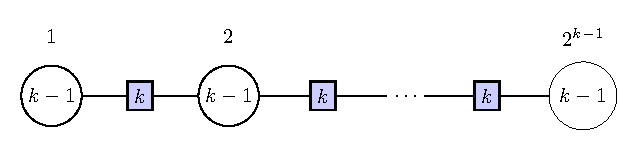
\includegraphics[scale=1]{pictures/t3/km1_c.pdf}
\end{figure}

Veamos que si unimos cada par de vértices vecinos como se realiza en la \textbf{\figref{fig:ej3}}, generamos un camino que se ve como el siguiente:

\begin{figure}[h]
  \centering
  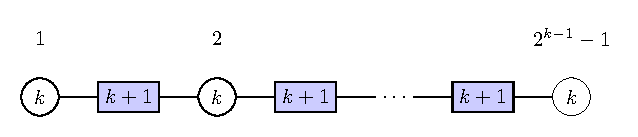
\includegraphics[scale=1]{pictures/t3/km1.pdf}
\end{figure}

El camino generado tras unir los vértices vecinos del grafo $G_{(k-1)}$ es parecido al camino generado por $k$, con la diferencia de que tiene $2^{k-1}+1$ nodo menos. Por tanto la palabra que se va a generar por este camino le está faltando 1 elemento de $\Sigma^k$, por lo que no es $k-$completa. Finalmente, el largo de la palabra que se generará con esté camino es de $2^{k} $. Por tanto, en el grafo para construir la palabra $(k-1)-$completa no es posible obtener una palabra $k-$completa. 

Por la parte 3 sabemos que existe una palabra $(k-1)-$completa cuyo largo es menor a $2^{(k-1)+1} + (k-1) - 1 =2^{k} + k - 2 $. 

\begin{figure}[h]
\centering
\begin{minipage}[b]{0.4\linewidth}
\centering
\begin{tikzpicture}[rotate=-45]
  \GraphInit[vstyle=Simple]
  \SetVertexSimple[MinSize=5pt]
  \renewcommand * {\EdgeLineWidth}{0.5pt}
  \Vertices{circle}{A,B,C,D}
  \Edges[style={{Triangle[angle=45:5pt]}-{Triangle[angle=45:5pt]}}](C,B,A,D,C,A,D,B)
\end{tikzpicture}
\caption{Grafo dirigido general}\label{fig:dirig_total}
\end{minipage}
\hspace{3cm} % Cambiar este espacio
\begin{minipage}[b]{0.4\linewidth}
\centering
\begin{tikzpicture}[rotate=-45]
  \GraphInit[vstyle=Simple]
  \SetVertexSimple[MinSize=5pt]
  \renewcommand * {\EdgeLineWidth}{0.5pt}
  \Vertices{circle}{A,B,C,D}
  \Edges[style={-{Triangle[angle=45:5pt]}}](C,B,A,D,C)
\end{tikzpicture}
\caption{Circuito euleriano conveniente, sin pesos}\label{fig:camino_util}
\end{minipage}
\end{figure}